\chapter{Introduction}
\label{chap:intro}
\minitoc
\section{Context}

Making sense of texts plays a vital role on the evolution of general artificial intelligence. Given the constantly-growing generation of textual data, there is the need of computational systems able to extract useful information from large quantities of textual collections, mainly to facilitate our day-to-day activities and, not less important, to find useful latent information hidden behind these large quantities of data. For example, Google, the search engine giant, is now able to conveniently answer short questions by analyzing textual knowledge bases, such as the English Wikipedia, in order to find the answer. Furthermore, Gmail, the Google's electronic mail interface, now  automatically identifies events, and sometimes their location and participants, from our personal emails and then adds  them to our online agendas. On the other hand, finding latent correlations within entities described in the text [example]

Indeed, making computers learn,  via theories, algorithms and applications, is the general objective of artificial intelligence research. Coming from this multi-disciplinary area, Natural Language Processing\footnote{And its more applied branch, text mining or text analysis. While it is sometimes argued that text mining deals with the structured data information extracted from text, I believe both terms considerably overlap nowadays. For ease of readability, in this dissertation we use both terms interchangeably, while preferring Natural Language Processing.} (NLP) is the domain that aims to make machines understand our language. Specifically, speech and text, the latter being the focus of this work.

NLP has developed rapidly during the last two decades mainly due to the combination of three factors: 
\begin{itemize}
\item The  availability of \textbf{large quantities of freely-accessible textual data}: primarily enabled by the current Web technologies, we are today able to download with a single click the entire content of the English (or other languages) Wikipedia. In the same sense, we can also download thousands of gigabytes of Web crawled data. This information is used to derive knowledge about the text itself, as we will see in the rest of this dissertation. 
\item The \textbf{computational power} at our disposition: from consumer-based computers able to perform parallel computations with considerably large datasets; to on-demand distributed cloud platforms with high performance computing nodes. The latter may be from private providers, e.g., AWS Cloud Service\footnote{\url{https://aws.amazon.com/}}, Microsoft Azure\footnote{\url{https://azure.microsoft.com/en-us/}}, etc; or furnished by public organizations, such as France's Lyon 1 University\footnote{\url{https://p2chpd.univ-lyon1.fr/}} or the National Institute of Nuclear Physics computing centers\footnote{\url{https://cc.in2p3.fr/}}.

\item  The \textbf{large quantity of open-source text mining and data science analysis tools}. Luckily, it is becoming more common for NLP laboratories around the world to make their developments available to the general public, e.g, Stanford University CoreNLP\footnote{\url{https://stanfordnlp.github.io/CoreNLP/}}, Antwerp's University CLiPS Pattern\footnote{\url{http://www.clips.ua.ac.be/pattern}}.
% Paris 7's University Alpage Team Software\footnote{\url{https://www.rocq.inria.fr/alpage-wiki/tiki-index.php?page=Logiciels}}. 
Additionally, large Web companies, such as Facebook\footnote{\url{https://github.com/facebookresearch}} and Google\footnote{\url{https://github.com/google}}, frequently publish their research code and utilities. Lastly, communities of individuals develop libraries that grow to become essential building blocks of several applications and research in the domain. Notably, \texttt{scikit-learn}\footnote{\url{http://scikit-learn.org/}}, a popular data science library implementing several well-known machine learning algorithms. Regarding NLP specifically, two up-to-date libraries stand out:  \texttt{gensim}\footnote{\url{https://radimrehurek.com/gensim/}} and \texttt{spaCy}\footnote{\url{https://spacy.io/}}. These are, for the most part, cross-platform, high performance, optimized, well maintained, documented, easily installable and open source libraries.
% The former specializing on topic modeling and the latter on word's distributional representations.

\end{itemize} 
\begin{figure}
\centering
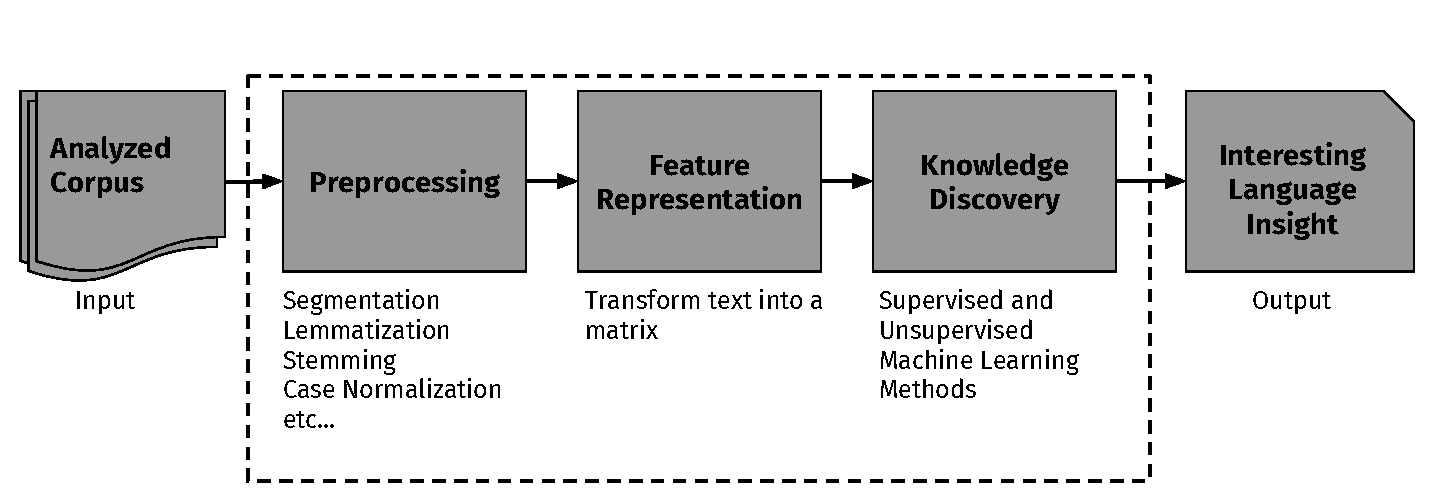
\includegraphics[width=1\linewidth]{./images/Chapitre1/nlp_flow.pdf}
\caption{Typical steps of Natural Language Processing applications.}
\label{fig:nlpflow}
\end{figure}
NLP tasks generally follow the same procedure to achieve their respective goals. First, starting with an input corpus (already collected before), a NLP system first preprocess the data in order to "normalize" the input raw text. Secondly, in Feature Representation, a large number of features is extracted from the text. Thirdly, in Knowledge Discovery,  a machine learning or rule-based (less common nowadays) technique is used to  learn a model able to provide an interesting insight on the existing data as well as on new instances.. The output of said system is usually the model or the language insight that reveals an interesting piece of information contained in the input corpus. Figure \ref{fig:nlpflow} describes the steps of a NLP system. 

Natural Language Processing is used today for several practical applications. From the elementary tasks that serve as the building blocks of more sophisticated systems to solving more advanced challenges. For example, in elementary tasks we have for example Part-of-Speech (PoS) tagging, a syntactic-grammatical task that aims to automatically determine grammatical tags for each word [?]; or Word Sense Induction and Disambiguation (WSI/WSD) which tries to determine and assign the correct sense for a word. Named Entity Recognition, or NER, another important task, which assigns aims to assign named entities with a type, in other words, discover if a proper noun is a place, or a person or an organization or any other type required by the application. 

More complex tasks that would ideally apply one of the mentioned tasks in order to get more precise knowledge about what is being talked about in the text. Sentiment analysis (or sentiment classification) is such task. The ultimate goal of this task is to determine the positiveness or negativeness expressed in a text. In this case, it would be useful to know what words express a ``sentiment'': usually adjectives, found via PoS tagging. Likewise, it would be informative to know what (or about who) we are talking about (with NER tagging) as well as the specific context that it is being discussed (WSI/WSD). 



\section{Challenges and Contributions}
There are several research challenges that arise from the choices taken in each one of the above mentioned steps. In this thesis,\textbf{ we particularly focus} on three challenges arising in both the \textbf{Feature Representation} and \textbf{Knowledge Discovery} phases:
\begin{enumerate}
 \item  Modeling, extracting, and efficiently storing different linguistic features coming from raw text,
 \item Leveraging links, and thus the structure, between text units in order to discover their latent relations, 
 \item Dealing with the sparseness inherent to text data while successfully combining the different available text features, 
\end{enumerate}

In that sense, the contributions that we propose to are the following:

\begin{figure*}
\centering
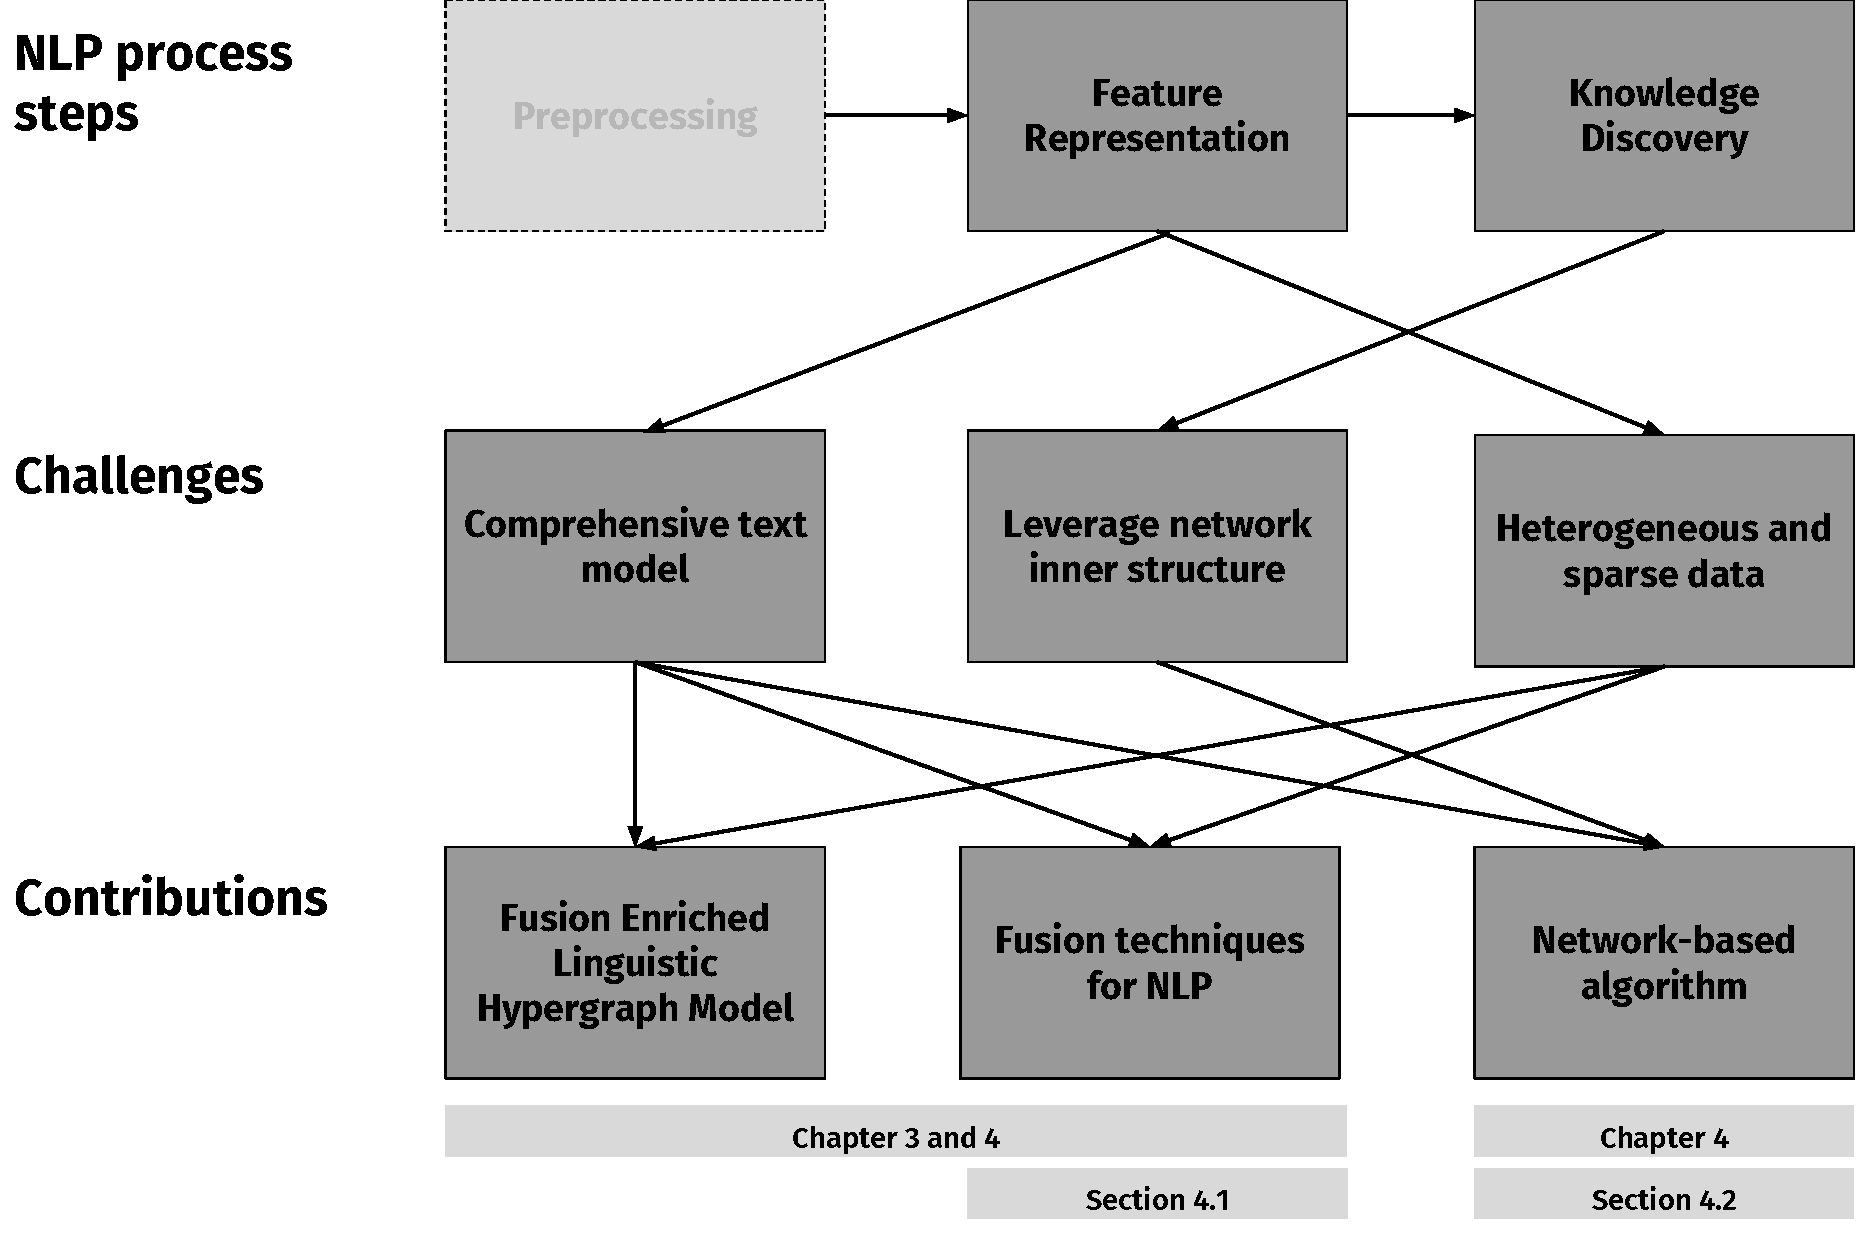
\includegraphics[width=1\linewidth]{./images/Chapitre1/challenges_contribs.pdf}
\caption{}
\label{fig:challenges_contribs}
\end{figure*}

 Below, we introduce each step as well as its characteristics:

\paragraph {Preprocessing}  According to the final application of the system, we deal with "irregularities" present within the text, so that we can extract more informative features from it. Conventional techniques include conflating (or blend) words according to their stems (stemming), conflating words with respect to their lemmas (lemmatization), removing functional words (articles, determinants, etc.), case normalization, replacing numeric tokens with strings, among others.

\paragraph {Feature Representation} In data analysis we often hear the saying "Garbage In, Garbage Out". Indeed, knowledge discovery (i.e., machine learning methods)  can only do so much with the input data they are given.  This step is then crucial for any NLP or data mining system.   During this step we transform each textual unit from the input corpus into a numerical representation (i.e., a matrix) that is compatible with the machine learning methods used in the following step.
%As we will see below, this dissertation focus on the challenges and opportunities this step presents. 

\paragraph {Knowledge Discovery} Several NLP tasks can be seen, directly or indirectly, as tasks assigning labels to words \cite{Collobert2011}. In that sense, machine learning methods are used to solve this kind of problems and thus are naturally used to solve most NLP problems nowadays. Either supervised learning (leveraging annotated corpora) or unsupervised learning (finding related elements within the text, without any extra information), the goal is always to find interesting insights from the input corpus, towards a general language understanding. 
\\ \\
In this thesis we focus on the decisions and limitations that arise within the \textbf{Feature Representation} and \textbf{Knowledge Discovery} stages of the NLP systems flow. In the following paragraphs we will discuss   the challenges that motivate our contributions.

\section{Challenges and Contributions}
Concerning Feature Representation, there are three decisions that must be considered when creating a NLP system: 
\begin{enumerate}
\item The text-unit we want to work with (i.e., the text unit we want to represent). For exmaple, either words, sentences, paragraphs, etc.
\item The linguistic role of the text unit we want to analyze (e.g., word and phrase neighbors, syntactic relations);
\item The importance of each feature,  determined by a weighting scheme

\end{enumerate}

The systems that we build in this work require the representation of single words, that is our text unit is always defined to be a single word. The selection of weights is a matter of changing 

\textbf{Feature Representation} entails the definition 

%	Today, there are more than four billion pages indexed on the Web. Among these pages, it is argued that  70\%  of them consist of non-structured data, generally known as textual information. Thanks to the pervasiveness of computers and the Internet,  organizations are constantly generating  textual content. The entire English version of the Wikipedia encyclopedia has an ever-growing size of more than 16 Gb consisting of text. the community contributes daily to increase an improve the quality of the text (and hopefully the quality of the content).
% On the other hand, the CommonCrawl WWW repository contains X Tb of the Web's textual data. While the quality of the former example is not curated (it contains text from any kind of Web page) it proves to be useful simply by means of the quantity of it. 
%
%Alongside the development of community-driven creation of content on the Web, we find the effort put forward to design and implement open source data analysis tools.  These sophisticated off-the-shelf applications and libraries help us study the data through Data Mining, and more concisely, Natural Language Processing (NLP) techniques.


These last two factors, copious amounts of accessible data and open-source analysis tools coupled to computational prowess yields the opportunities that actually push research efforts in the area.
 A practical question that follows is how do we extract the useful meaning or knowledge latent within the text. 
 Briefly, to analyze textual data, we need to represent textual units (e.g.,  words, sentences, paragraphs, documents)   by means of features that describe them. 
 Moreover, text may be represented from different points of view. For example, we can characterize words with respect to its neighboring words or to the syntactical relations it appears in, or its role in the structure of a phrase, and so on. Each one of these dimensions distinguishes a given word in different useful ways and more importantly they also complement each other. We argue that in order to thoroughly analyze text,  we need a multi-layered model able to take into account these levels of representation in order to find complementary relatedness among  text during the analysis.

The  large amount of text data plus the need to represent it as globally as possible poses non-trivial challenges for comprehensive textual analysis. Firstly, we need an efficient and straight-forward model to store heterogeneous textual information and the links within it. Secondly, we require efficient algorithms that take advantage from the information stored. Thirdly, we require to leverage the diversity of the representations by finding complementary ways textual units interact among them. 
%In other words, on the one hand we need a model able to hold linked and heterogeneous linguistic information, on the other hand, we need efficient analysis techniques that are also able to leverage latent interactions between textual features.

\begin{figure}
\centering
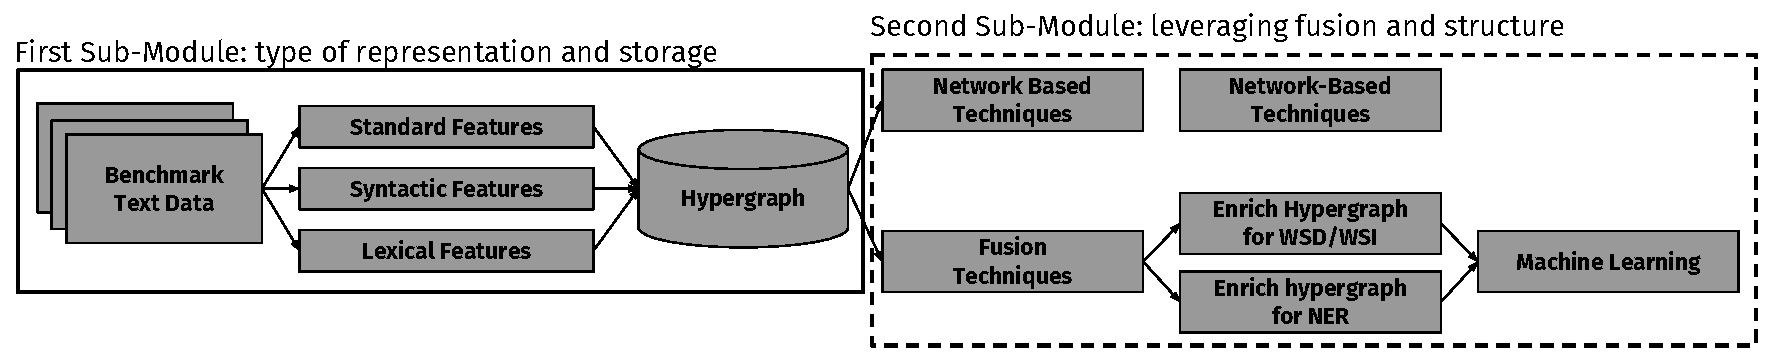
\includegraphics[width=1\linewidth]{./images/Chapitre1/main_diag2.pdf}
\caption{Modular description of this dissertation}
\label{fig:maindiag}
\end{figure}


In the literature, language representation models are generally based on two types: the vector space model and the network (or graph) model. The former represents textual units through their features in a vector space. The latter represents the interactions between textual units in a graph-based by means of nodes and edges. In the end though, both representations are intertwined as we can represent a graph as an object-feature matrix through its incidence or adjacency matrices.

%In this thesis we focus on solving NLP applications while using a language network to represent textual features.


Language (or linguistic in this thesis) networks  have been studied profoundly. Its theory draws heavily from several research fields (complex networks, graph theory, linguistics, natural language processing). Using the division proposed by \cite{Choudhury09}, in the related literature, works follow one of two directions: they analyze the nature of the network from a structural point of view (citations here); or they leverage the network to solve NLP tasks (citations here). The second direction can be further divided into two sub-classes: those that contain homogeneous textual features; and those that comprise heterogeneous descriptors (citations here). In the majority of these works, we note two main shortcomings:
\begin{enumerate}
\item the majority of related works that deal with the application of language networks do not take into consideration different types of feature representations. Having a global insight into textual data allows for deeper structural and application analysis.
\item the works that do implement heterogeneous solutions, do not aim to explicitly profit from the complementarity of the features diversity. Finding relatedness between textual units at different levels of representation can be useful to improve the results of NLP applications.
%\item There is not an explicit use of background data, that is,  open sources of textual data are notleverage

\end{enumerate}
 

The main topic of this dissertation is language representation through a heterogeneous linguistic network and its applications on NLP. Our objective is twofold: first, to conceive a model able to handle multiple textual-data features extracted from. Second, to use this model to solve NLP tasks efficiently and making explicit use of the features diversity. Furthermore, we aim to leverage open-source corpus to complement in-domain datasets.  To achieve our goals, we base our model, and proposed applications, on five main concepts: linguistic representations, the distributional hypothesis, network analysis (and related methods),  multimedia fusion techniques, and lastly,  machine learning methods, namely supervised and unsupervised approaches. these techniques are used as the tools to fit learning models over our data. Indeed, to accomplish the second goal,  we propose solutions to two well-known natural language processing tasks: word sense induction and disambiguation and named entity recognition. 

%Below I introduce both theoretic concepts and NLP applications studied in this work.

%given an input corpus, we conceive and implement a language network model that represent lexical, syntactical, and orthographic contextual features for each word.  Next, we propose an algorithm that leverages the internal network structure to determine the correct sense of a target word, namely the word sense induction and disambiguation task. Finally, we combine the features contained in the network in order to find out we are able to compute semantic relatedness among them by means of similarity their contexts.
% distributional hypothesis. In short, the distributional hypothesis states that we are able to estimate the semantics of words from the analysis of their contexts.
%




%  The answer lies on a well-known model: the distributional model. Briefly, the distributional model states that the semantic similarity between words can be determined from the distribution of their contexts. In other words, two words sharing a similar context (a context being the surrounding words, for example) will share a similar meaning. The distributional model is nowadays one of the core principles that guide NLP experiments and research \cite{di2013clustering}.


\section{Contributions}
Having cited the disadvantages of current language representations and applications, we set out to fill the gaps with our own propositions. First, in order to have a dataset to test and work with, we parsed and stored the English Wikipedia taking into account largely-ignored syntactic information. Secondly, we fitted our linguistic network to a sample of the parsed Wikipedia corpus. Thirdly, we proposed an algorithm to solve word sense induction and disambiguation by leveraging the network's structure. Finally, we present a method that combines textual features to solve both named entity recognition and again word sense induction and disambiguation. More concisely, we make the following contributions in this dissertation:
\begin{itemize}
\item An annotated parsed dump of the English Wikipedia. In this parse we focus  onto the syntactical characteristics of words: aside from the classical Part-of-Speech (PoS) tags and dependency parsing relations, we provide the full constituent parse branch for each word in a succinct way.  
\item Using the information extracted in the previous step, we propose a heterogeneous language network that takes into account lexical and syntactical linguistic information. The proposed model aims to take advantage of the information stocked within our dump and to overcome the limitations of current language networks. We propose a novel hypergraph model able to link together words according to different characteristics. 
\item An algorithm that leverages  the structure of the network in order to solve word sense induction and disambiguation. Our proposed method takes into consideration the "real-world" characteristics of the graph to group similar senses and then assign them to target words. We  improve the overall performance compared to other similar graph-based techniques.
\item We explore multimedia fusion techniques to complement the features hold by the network. Specifically, we focus on solving named entity recognition and word sense induction and disambiguation by applying feature-combination methods that have already shown their efficiency in the multimedia analysis domain.  Our results show that the combination of textual features indeed improves the performance compared to single feature representations and trivial features concatenation. Even more, we experiment with background information from open text sources to further improve the performance of our models. Finally, we also present an analysis on the behavior of features according to different types of senses and entity classes.


\item   We render public our parsed Wikipedia dump as well as the tools (and its source code) used to perform the parse. The implemented methods are also freely available.


\end{itemize}

\section{Structure of the Dissertation}
The remainder of this thesis is structured as follows:
\paragraph{Chapter \ref{chap:backgnd}} This chapter has a detailed overview about the first four axes of this thesis: how we can represent words from a lexical, syntactic and semantic point of view, then, how we find relatedness among words based on  the distributional hypothesis, and how we link both words and features together in a language network to discover their structure and to extract useful knowledge. 
%
%Afterwards, we present how these features can be combined to improve the results of single-feature based solutions. 
Afterwards, we detail the machine learning methods used to solve the NLP tasks. Finally, we present the two NLP tasks we solve using our propositions: Word Sense Induction and Disambiguation (WSI/WSD) and Named Entity Recognition (NER).
\paragraph{Chapter \ref{chap:related_wk}} We discuss previous work related to the main contribution of this work, linguistic networks. We cover the previous work specific to each task in its corresponding chapter.

\paragraph{Chapter \ref{chap:ling_net}} We present and define a novel structure to hold language information: the hypergraph linguistic model.  We discuss its characteristics and the intuitions behind its conception: the hypergraph choice,the role of nodes and edges, the type of features stored, the advantages it present in terms of accessing and manipulating the data. In the following chapters, we address the applications that leverage the properties of the structure proposed.

\paragraph{Chapter \ref{chap:wsd}} In this chapter, we present an algorithm that exploits the structure of the network, i.e., the connections between nodes. Namely, we derive senses from a test corpus by finding related words connected to a single main node. We test the linguistic and lexical features and discuss about its qualities. Our results improve on the performance of similar propositions from the literature. We study the combination of features using multimedia fusion techniques in the next chapter.

\paragraph{Chapter \ref{chap:fusion}} We explore the application of multimedia fusion techniques using linguistic features to solve NLP tasks. Briefly, fusion techniques may consist on trivially concatenating feature columns or a combination that aims to transfer relatedness information from one representation to a second one. We experiment with these methods on three datasets for named entity recognition and one dataset for word sense induction and disambiguation. Indeed, we show that using certain configurations of fusion techniques can lead to improvements over single-feature and trivial-concatenation representation matrices. Furthermore, we explore the contribution from each representation kind to each sense and class in each task respectively.
\paragraph{Chapter \ref{chap:dump}} This chapter describes the process of parsing and storing an English Wikipedia Syntactical Dump. We use open source tools on freely available data to generate a software that is able to extract lexical and syntactic data from a given corpus.We thus create and publicly release a syntactically annotated version of the English Wikipedia containing often-neglected information, stored in a format that facilitates its manipulation. 

\paragraph{Chapter \ref{chap:conclusions}} We conclude this dissertation and present possible avenues for future work.

